Bla bla bla...

% \begin{figure}
    % 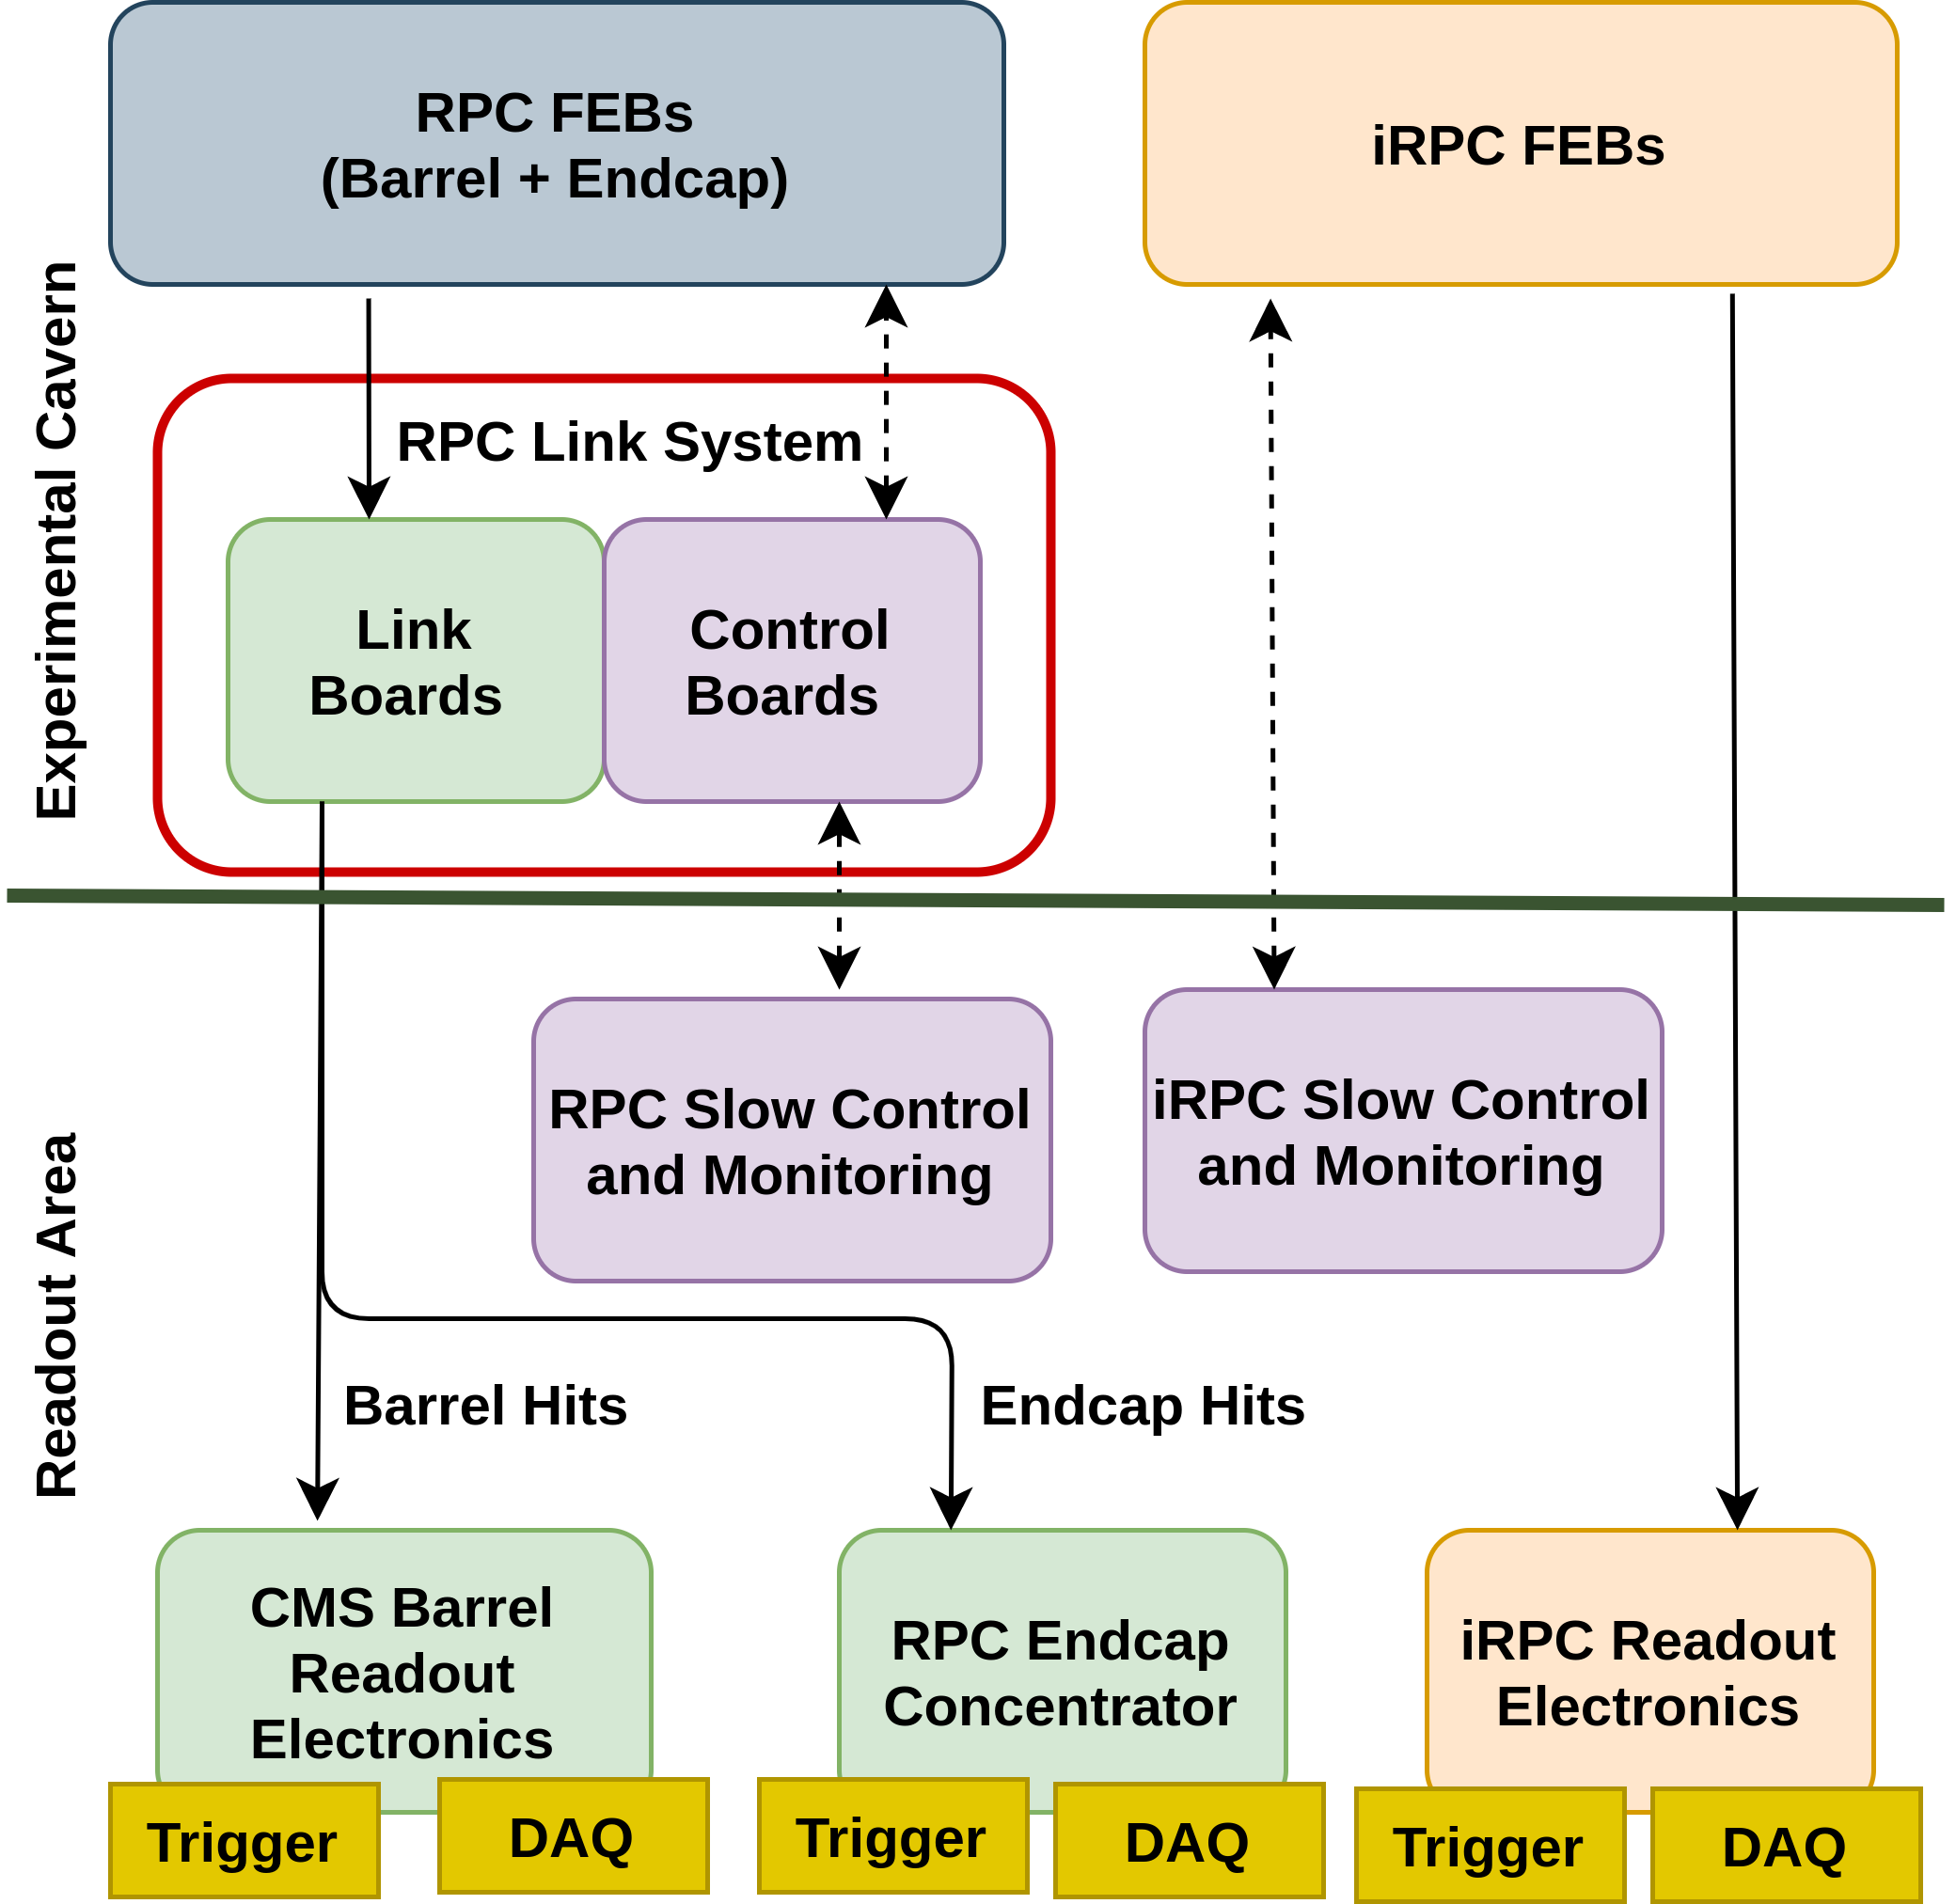
\includegraphics[width=0.5\textwidth]{uioposter-images/rpc_phase2_readout.png}
    % \caption{A quadrant of the CMS Muon Spectrometer, showing DT chambers (yellow), RPCs (light blue), and CSCs (green). The locations of new forward muon detectors for the HL-LHC project are contained within the dashed box and indicated in red for Gas Electron Multiplier (GEM) stations (ME0, GE1/1, and GE2/1) and violet for improved RPC stations (RE3/1 and RE4/1).}
%     \label{cms_muon_upgrade}
% \end{figure}

\begin{wrapfigure}{r}{0.5\textwidth}
    \caption{A capition for RPC readout}
    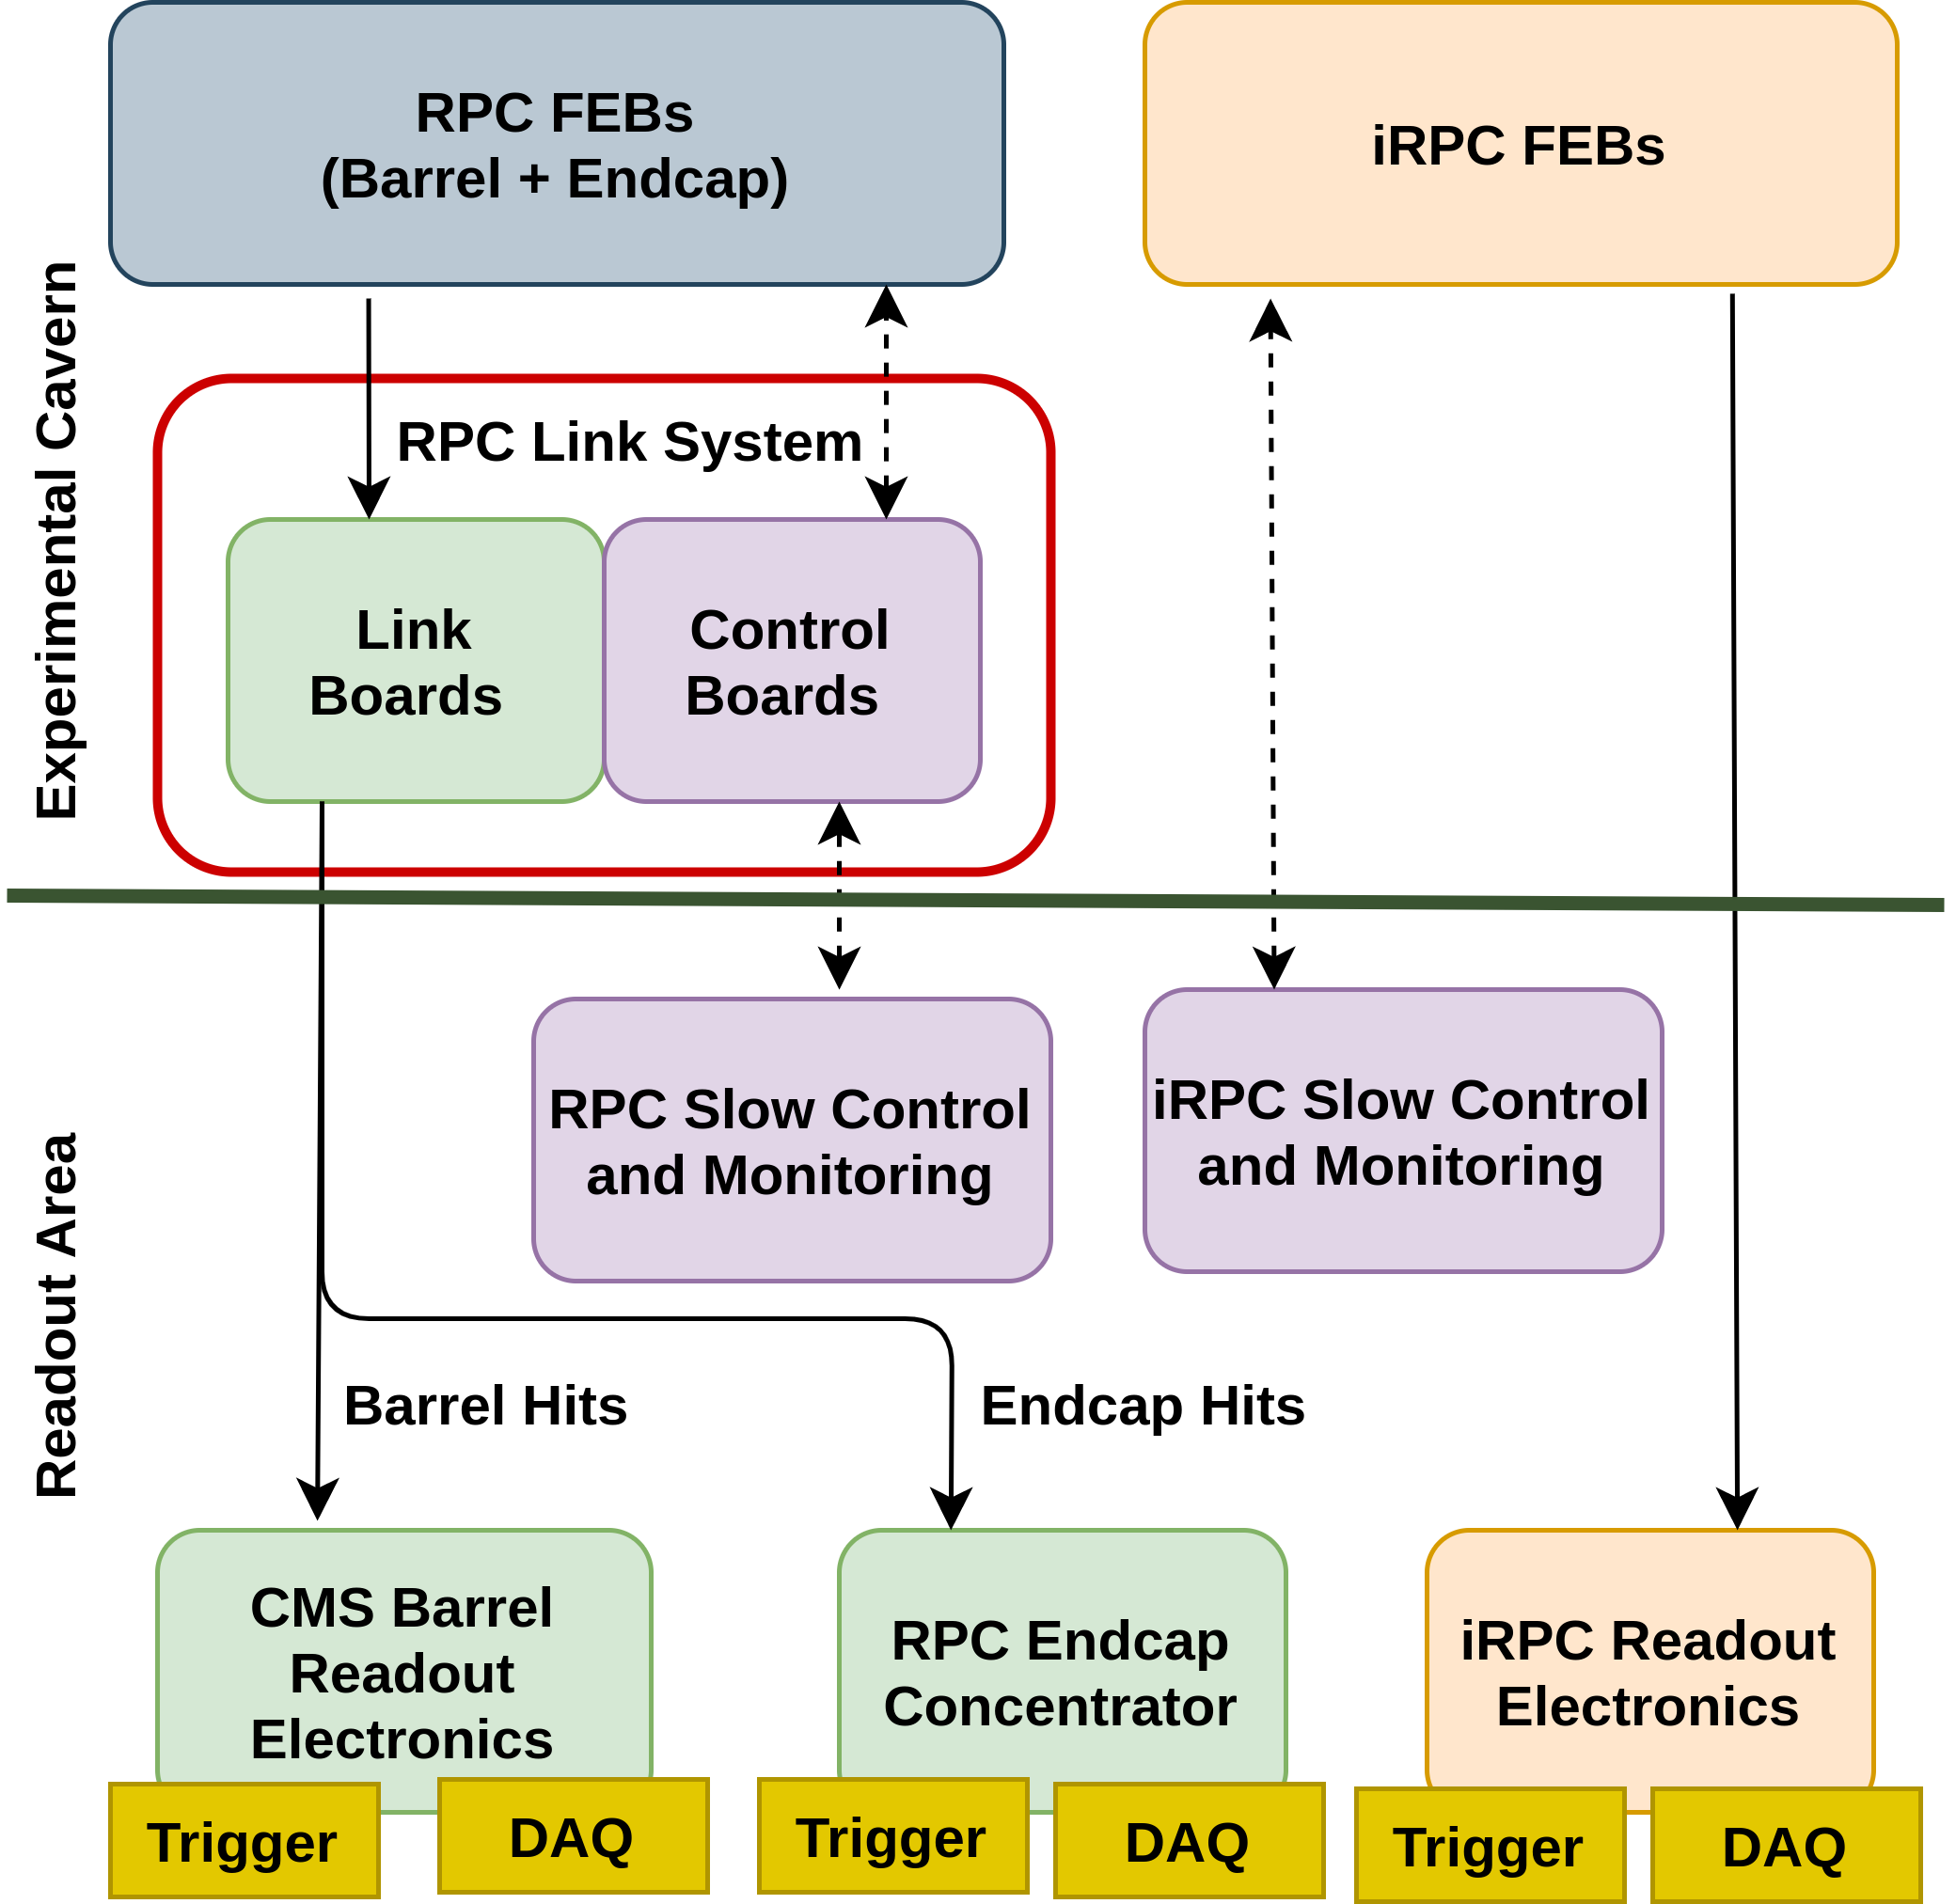
\includegraphics[width=0.5\textwidth]{uioposter-images/rpc_phase2_readout.png}
    \label{rpc_phase2_readout}
\end{wrapfigure}


Bla bla bla... Bla bla bla... Bla bla bla... Bla bla bla... Bla bla bla... Bla bla bla... Bla bla bla... Bla bla bla... Bla bla bla... Bla bla bla... Bla bla bla... Bla bla bla... Bla bla bla... Bla bla bla... Bla bla bla... Bla bla bla... Bla bla bla... Bla bla bla... Bla bla bla... Bla bla bla... Bla bla bla... Bla bla bla... Bla bla bla... Bla bla bla... Bla bla bla... Bla bla bla... Bla bla bla... Bla bla bla... Bla bla bla... Bla bla bla... Bla bla bla... Bla bla bla... Bla bla bla... Bla bla bla... Bla bla bla... Bla bla bla... 

Bla bla bla... Bla bla bla... Bla bla bla... Bla bla bla... Bla bla bla... Bla bla bla... Bla bla bla... Bla bla bla... Bla bla bla... Bla bla bla... Bla bla bla... Bla bla bla... Bla bla bla... Bla bla bla... Bla bla bla... Bla bla bla... Bla bla bla... Bla bla bla... Bla bla bla... Bla bla bla... Bla bla bla... Bla bla bla... Bla bla bla... Bla bla bla... Bla bla bla... Bla bla bla... Bla bla bla... Bla bla bla... Bla bla bla... Bla bla bla... Bla bla bla... Bla bla bla... Bla bla bla... Bla bla bla... Bla bla bla... Bla bla bla... 